\chapter{Introduksjon}
%--------------------MÅ INN I HOVEDRAPPORT------------------------------------------
\fixme Rotårsaksanalyser er et lite brukt verktøy innen informasjonssikkerhet, men er av økende betydning. Vanlig tilnærming til informasjonssikkerhetsstyring er å utføre en risiko-og sårbarhetsanalyse (ROS-analyse) for så å gjennomføre tiltak som fører risikoene til et akseptabelt nivå. En annen hyppig brukt tilnærming er hendelseshåndtering der en planlegger hvordan det skal responderes på hendelser etter de er inntruffet. Rotårsaksanalyse skiller seg fra disse ved å gå i dybden på problemet, kartlegge hva slags rotårsaker som står bak, og innføre tiltak for å fjerne disse helt.
%%%%%%%%%%%%%%%%%%%%%%%%%%%%%%%%%%%%%%%%%%%%%%%%%%%%%%%%%%%%%%%%%%%%%%%%%%%%%%%%%%%%%

\section{Oppgavebeskrivelse}
Denne rapporten er en delrapport i en større oppgave om rotårsaksanalyse. Dette caset går inn på rotårsaken til at skolen har mye passord og brukernavn som på avveie. I denne rapporten bruker vi kompromittert bruker, da mener vi at passord og brukernavn har kommet på avveie. Vi ser i denne rapporten kun på ansatt sin brukerkonto og ikke studentkonto, da studentkonto ikke har like mye rettigheter som ansatte.

I 2017 var kompromitterte kontoer alene årsaken til ca. 70 sikkerhetshendelser ved NTNU. I desember 2017 kom det også en stor datadump som innholdt over 5000 kontoer affiliert med NTNU, som alle innehold passord og brukernavn. Av disse var det 101 som fortsatt var aktive i systemene til NTNU. 

En del av kompromitterte kontoer blir brukt av utenlandske aktører for å få tilgang til forskningsartikler, noe som koster skolen vår rundt (50?) dollar per artikkel. Av slike artikler, blir det hentet ut flere tusen av på en gang per bruker. Skolen vet ikke om når det blir hentet ut artikler, eller om det er legitimt bruk av artikler, de får ofte vite det først når skolen får beskjed av samarbeidspartnere til NTNU, for eksempel de som tilbyr artiklene. 

Denne analysen går ut på å identifisere rotårsaken til hvorfor NTNU har så mange kompromitterte brukerkontoer.


\section{Metode}

Metodebruken i denne analysen er delt inn i syv steg som vist i \hyperref[fig:prosess]{Figur 2} under. I hvert steg av denne prosessen brukes det ulike verktøy for å hjelpe til med å forstå problemet, finne rotårsak, og tilslutt implementere tiltak for å eliminere årsakene. 
\begin{figure}[H]
    \centering
    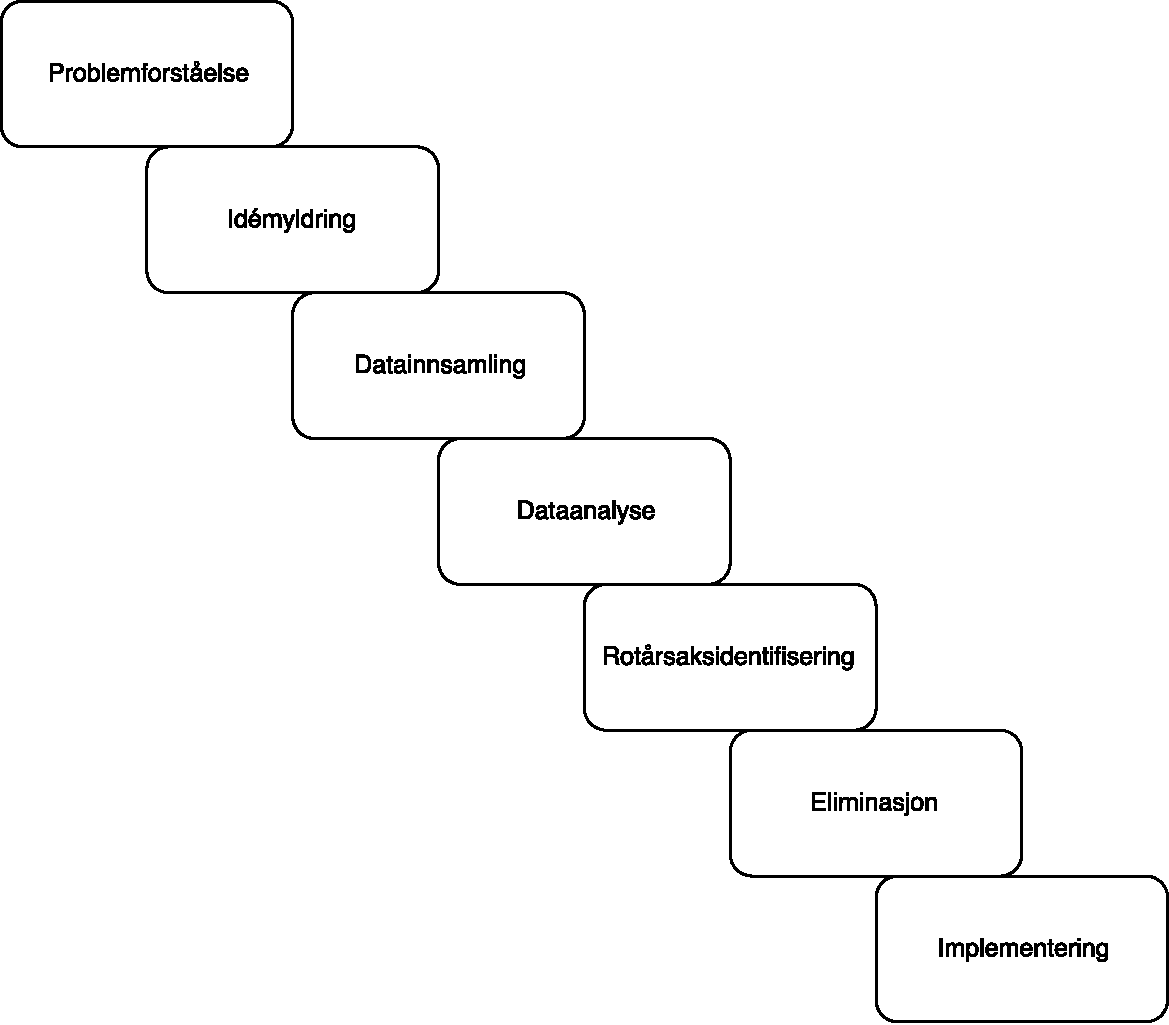
\includegraphics[scale=0.6]{case_1/bilder/prosess.pdf}
    \label{fig:prosess}
    \caption[Rotårsaksanalyseprosessen]{Rotårsaksanalyseprosessen definert av Andersen og Fagerli}
\end{figure}